\documentclass[10pt,a4paper]{article}

\usepackage[a4paper,margin=20mm]{geometry}
\usepackage{graphicx}
\usepackage{subcaption}
\usepackage{booktabs}
\usepackage{amsmath}
\usepackage{url}
\usepackage{float}
\usepackage{placeins}
\usepackage[hidelinks]{hyperref}
\usepackage{tabularx}
\usepackage{array}

\title{Failure Case Analysis and Reliability Improvement of SegFormer-B0 for Semantic Segmentation}
\author{
Name: Luna Sugiyama \\
Student ID: 48-256422 \\
Department: Information Electrical Communication Engineering \\
Laboratory: Sugiura Lab. \\
}
\date{}

\begin{document}
\maketitle

\begin{abstract}
This report analyzes SegFormer-B0, a lightweight Transformer-based semantic segmentation model.
Instead of only reproducing the original model, the goal is to run the model, identify failure conditions, and propose practical improvements.
I use the pretrained SegFormer-B0 model fine-tuned on ADE20K and evaluate it on urban scene images and out-of-distribution objects.
The first failure case focuses on objects whose semantic category is not included in the ADE20K label set.
In particular, vending machines are visually recognizable to humans, but SegFormer-B0 cannot output the class ``vending machine'' because the class is absent from the model's predefined output labels.
The second failure case focuses on thin-object disappearance, where the target class exists in the label set but is not predicted in the selected region.
Based on these analyses, I propose class-set-aware and missing-target failure warnings to make silent segmentation failures visible to users.
\end{abstract}

\section{Introduction}

Semantic segmentation is a fundamental task in computer vision where each pixel in an image is assigned a semantic class label.
It is widely used in autonomous driving, robotics, surveillance, augmented reality, and visual media analysis.
Recent Transformer-based models have achieved strong performance, but practical deployment still faces reliability problems.
In real images, a model can fail due to low image quality, domain shift, unusual viewpoints, small objects, or semantic categories that are not included in the training label set.

This report studies these problems using SegFormer-B0.
The objective is not only to run an existing model, but also to analyze when and why it fails.
In particular, I focus on the following question:

\begin{quote}
Can a semantic segmentation model produce a visually plausible but semantically wrong output when the correct class is unavailable or difficult to detect?
\end{quote}

This question is important because a model with a fixed label set is forced to choose one of its known classes even when the input contains an unsupported object.
Furthermore, even when the correct class exists, small or thin objects may disappear into large surrounding classes.
As a result, the model may appear to work while silently producing an incorrect interpretation.

\section{Source Code}

The source code used for the experiments is available on GitHub:

\begin{quote}
\url{https://github.com/LunaSugiyama/masters/tree/main/m2/mon4visualmedia}
\end{quote}

The repository contains the SegFormer inference scripts, ROI-based failure analysis scripts, generated result images, and tables used in this report.

\section{Target Paper}

The target paper is:

\begin{quote}
Enze Xie, Wenhai Wang, Zhiding Yu, Anima Anandkumar, Jose M. Alvarez, and Ping Luo, 
``SegFormer: Simple and Efficient Design for Semantic Segmentation with Transformers,'' 
NeurIPS 2021.
\end{quote}

SegFormer is a semantic segmentation framework that combines a hierarchical Transformer encoder with a lightweight all-MLP decoder.
Unlike earlier segmentation models that rely heavily on convolutional decoders, SegFormer uses a simple decoder design while preserving multi-scale features from the encoder.
The model family includes several scales, from lightweight models such as B0 to larger models such as B5.
In this report, I use SegFormer-B0 because it is lightweight and can be executed on a CPU environment.

\section{Method Understanding}

SegFormer consists of two main components.

First, the encoder extracts hierarchical features from the input image.
Because the encoder is Transformer-based, it can model long-range visual dependencies while still producing multi-resolution feature maps.
This is useful for semantic segmentation because both local details and global context are important.
For example, pixels belonging to a road, building, or sky region can be recognized more reliably when the model understands the surrounding scene structure.

Second, the decoder maps the extracted features to pixel-level class predictions.
SegFormer uses a lightweight MLP decoder rather than a heavy convolutional decoder.
This design makes the model relatively efficient while maintaining good segmentation performance.

The pretrained model used in this report is:

\begin{quote}
\texttt{nvidia/segformer-b0-finetuned-ade-512-512}
\end{quote}

This model is fine-tuned on ADE20K and predicts one of the ADE20K semantic classes for each pixel.
Therefore, the output space is fixed.
If an object category is not included in ADE20K, the model cannot directly output that category.

\section{Implementation and Execution Environment}

The experiment was implemented in Python using PyTorch, Hugging Face Transformers, Pillow, NumPy, and OpenCV.
The environment was managed using \texttt{uv} to improve reproducibility.

\begin{table}[H]
\centering
\caption{Execution environment.}
\begin{tabular}{ll}
\toprule
Item & Value \\
\midrule
Language & Python 3.11 \\
Model & SegFormer-B0 fine-tuned on ADE20K \\
Framework & PyTorch, Hugging Face Transformers \\
Device & CPU \\
Environment manager & uv \\
Input image format & JPG, PNG, WebP \\
Output & Segmentation mask, overlay image, confidence map, ROI summary CSV \\
\bottomrule
\end{tabular}
\end{table}

For each input image, the script saves the original image, the predicted segmentation mask, an overlay visualization, a confidence map, and class distribution statistics.
For failure analysis, I additionally implemented a region-of-interest analysis script.
Given a manually selected bounding box around a target object, the script calculates the predicted class distribution and mean confidence inside that region.

\section{Baseline Experiment: Urban Street Scene}

As a baseline experiment, I applied SegFormer-B0 to a normal daylight urban street image.
The image contains common urban scene categories such as buildings, road, sky, trees, cars, sidewalk, and pedestrians.
The model produced reasonable segmentation for large semantic regions.
For example, the sky, buildings, road, trees, cars, and sidewalks were recognized as coherent areas.

However, the result also showed a limitation.
Small or thin objects such as traffic lights, road signs, poles, distant pedestrians, and tower structures were not segmented cleanly.
Some of these objects were absorbed into larger surrounding classes or fragmented into small regions.
This suggests that SegFormer-B0 is reliable for large scene-level categories but less reliable for fine structures and small objects.

\begin{figure}[H]
\centering
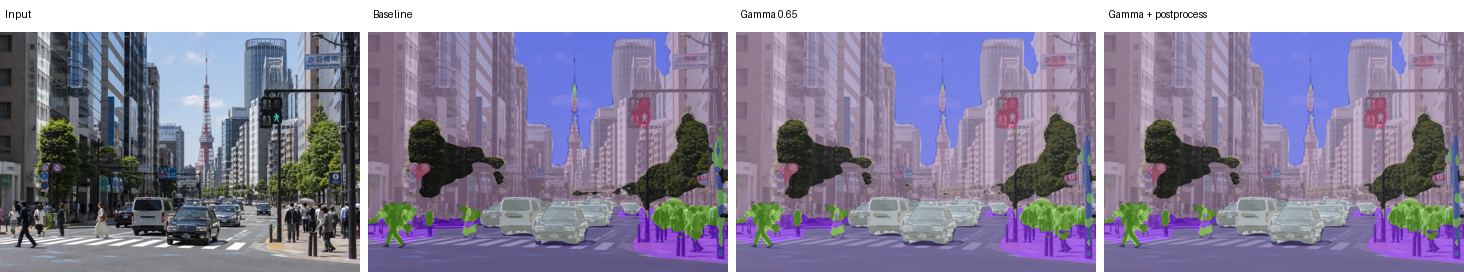
\includegraphics[width=\linewidth]{figures/comparison_overlay.png}
\caption{Baseline SegFormer-B0 result on a daylight urban street image. Large regions such as road, buildings, trees, and sky are recognized reasonably well, while small and thin structures are less stable.}
\label{fig:street_baseline}
\end{figure}

\FloatBarrier

\section{Failure Case 1: Out-of-Distribution Object Category}

\subsection{Motivation}

The first failure case is an out-of-distribution object category.
Here, ``out-of-distribution'' does not necessarily mean that the image itself is visually strange.
Instead, it means that the target object category is not included in the model's output label set.

I used vending machines as the target object.
Vending machines are common in Japanese urban scenes and are visually easy for humans to recognize.
However, the ADE20K label set used by SegFormer-B0 does not contain the exact class ``vending machine.''
Therefore, even when a vending machine is clearly visible, the model cannot output the correct semantic label.
It must assign the pixels to one or more existing ADE20K classes.

This is a label-space limitation rather than an image-quality problem.
Preprocessing such as brightness correction or denoising cannot create a missing semantic class.

\subsection{Verification Method}

To verify this failure, I used the following procedure.

\begin{enumerate}
    \item Check whether the target class ``vending machine'' exists in the SegFormer-B0 ADE20K label set.
    \item Manually select a bounding box around the vending machine region.
    \item Run SegFormer-B0 on the image.
    \item Calculate the predicted class distribution inside the selected region.
    \item Record the mean confidence inside the region.
\end{enumerate}

If the target class is absent and the pixels inside the object region are assigned to unrelated or substitute classes, the failure is verified.
This method is more precise than only looking at the full-image segmentation mask because it directly measures what the model predicts inside the object of interest.

\subsection{Results}

Table~\ref{tab:ood_vending_results} shows the ROI-based results for three vending machine images.
In all three cases, the exact target label ``vending machine'' was absent from the ADE20K label set.
The model therefore predicted alternative labels inside the vending machine region.

\begin{table}[H]
\centering
\caption{ROI-based analysis for vending machine images.}
\label{tab:ood_vending_results}
\small
\begin{tabularx}{\linewidth}{
    >{\raggedright\arraybackslash}p{0.18\linewidth}
    >{\centering\arraybackslash}p{0.20\linewidth}
    >{\centering\arraybackslash}p{0.20\linewidth}
    >{\raggedright\arraybackslash}X
}
\toprule
Image & Target label exists? & ROI mean confidence & Top predicted classes in ROI \\
\midrule
Vending 1 & No & 0.3844 & arcade machine, door, monitor, bulletin board, windowpane \\
Vending 2 & No & 0.5762 & wall, arcade machine, refrigerator, floor, bag \\
Vending 3 & No & 0.6021 & building, tree, booth \\
\bottomrule
\end{tabularx}
\end{table}

For Vending 1, the model predicted the region mainly as arcade machine, door, monitor, bulletin board, and windowpane.
This result indicates that the model interprets different parts of the vending machine as visually similar known categories.
For example, the illuminated display region can resemble a monitor, and the rectangular body can resemble a door or windowpane.

For Vending 2, the model predicted wall, arcade machine, refrigerator, floor, and bag.
This is particularly interesting because ``arcade machine'' and ``refrigerator'' are semantically closer to vending machine than many other classes, but they are still incorrect.
The model appears to map the unsupported object to the closest available categories in its label space.

For Vending 3, the selected region was predicted mainly as building, tree, and booth.
This result shows that the model can also be influenced by the surrounding scene and background.
Because the image contains vegetation and outdoor structures near the vending machines, the segmentation inside the ROI is mixed with surrounding categories.

\begin{figure}[H]
\centering
\begin{subfigure}{0.32\linewidth}
    \centering
    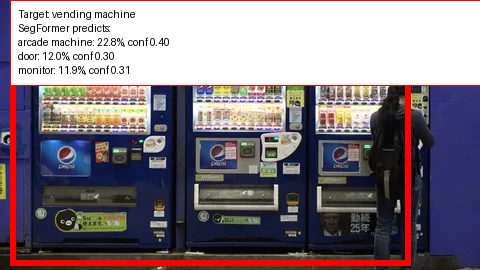
\includegraphics[width=\linewidth]{figures/vending_machine_1_roi.png}
    \caption{Vending 1}
\end{subfigure}
\begin{subfigure}{0.32\linewidth}
    \centering
    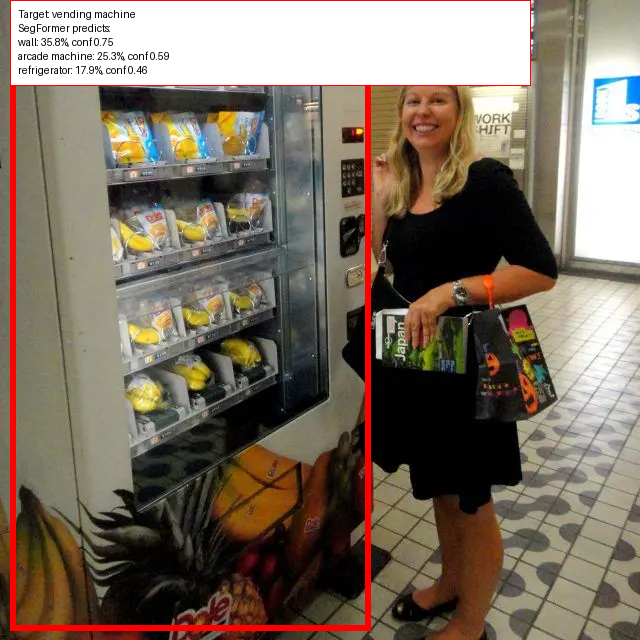
\includegraphics[width=\linewidth]{figures/vending_machine_2_roi.png}
    \caption{Vending 2}
\end{subfigure}
\begin{subfigure}{0.32\linewidth}
    \centering
    \includegraphics[width=\linewidth]{figures/vending_machine_3_roi.png}
    \caption{Vending 3}
\end{subfigure}
\caption{ROI visualizations for the vending machine failure case. The target object is clearly recognizable to humans, but the model assigns the region to existing ADE20K classes because ``vending machine'' is not included in the output label set.}
\label{fig:ood_vending_roi}
\end{figure}

\subsection{Analysis}

This failure case demonstrates a fundamental limitation of closed-set semantic segmentation.
SegFormer-B0 always predicts one of the ADE20K classes.
When the correct class is absent, the model cannot say ``unknown'' or ``unsupported.''
Instead, it assigns the pixels to the most visually similar available classes.

The vending machine examples show three important observations.

First, the failure is systematic.
The exact target class does not exist in the output label set, so the model cannot produce the correct label in any of the tested images.

Second, the wrong predictions are not random.
The model often predicts visually related categories such as arcade machine, refrigerator, monitor, door, or booth.
This suggests that the model has learned useful visual features, but its fixed label space prevents correct semantic interpretation.

Third, confidence alone is not a sufficient failure detector.
Although the ROI confidence is not extremely high in all cases, the model still gives concrete semantic labels instead of indicating that the object is unsupported.
A user looking only at the segmentation mask might incorrectly trust the result.

\FloatBarrier

\section{Improvement 1: Class-Set-Aware OOD Warning}

\subsection{Problem}

The OOD vending machine failure cannot be solved by simple image preprocessing.
The issue is not low brightness, blur, or noise.
The issue is that the correct class does not exist in the model's output label set.

Therefore, the improvement should not be brightness correction or mask smoothing.
A more appropriate improvement is to make the model's limitation visible to the user.

\subsection{Proposed Improvement}

I propose a class-set-aware OOD warning system.
Before trusting the segmentation result for a target object, the system checks whether the requested target class exists in the model's label set.
If the class is absent, the system displays a warning and reports the predicted surrogate classes inside the selected ROI.

For example, for the vending machine case, the improved system outputs:

\begin{quote}
Warning: ``vending machine'' is not included in the ADE20K label set.
SegFormer-B0 cannot output this class.
The selected region was instead predicted as arcade machine, refrigerator, wall, monitor, or booth.
The segmentation result for this object should not be trusted as a correct semantic label.
\end{quote}

This improvement does not add a new class to SegFormer-B0.
Instead, it improves reliability by preventing users from over-interpreting a closed-set segmentation output.

\subsection{Baseline vs. Improved System}

\begin{table}[H]
\centering
\caption{Comparison between baseline SegFormer-B0 and the improved OOD-aware system.}
\begin{tabular}{lll}
\toprule
Method & Output & User interpretation \\
\midrule
Baseline SegFormer-B0 & Predicts existing ADE20K classes & User may trust wrong labels \\
OOD-aware system & Shows unsupported-class warning & User knows the result is unreliable \\
\bottomrule
\end{tabular}
\end{table}

The proposed improvement is simple, but it directly addresses the failure mechanism.
Since the correct class is absent, a warning is more appropriate than post-processing the mask.
This turns a silent semantic failure into an explicit and interpretable system warning.

\FloatBarrier

\section{Failure Case 2: Thin Object Disappearance}

\subsection{Motivation}

The second failure case focuses on a thin tower structure in an urban street image.
Unlike the vending machine case, the target class \texttt{tower} exists in the ADE20K label set.
Therefore, this failure is not caused by an absent output class.
Instead, it is caused by the small and thin spatial structure of the object.

This case is useful because it tests a different limitation.
In the vending machine case, the correct label is unavailable.
In the tower case, the correct label is available, but the model still fails to predict it.

\subsection{Results}

I selected a bounding box around the tower and analyzed the predicted classes inside the ROI.
Although the tower is clearly visible to humans, SegFormer-B0 did not predict the class \texttt{tower} at all.
Instead, 57.3\% of the ROI was predicted as \texttt{sky}, and 40.9\% was predicted as \texttt{building}.
The mean confidence inside the ROI was 0.8069.

\begin{table}[H]
\centering
\caption{Baseline ROI analysis for the tower region.}
\label{tab:tower_failure}
\begin{tabular}{lrr}
\toprule
Predicted class & Ratio & Mean confidence \\
\midrule
sky & 0.5728 & 0.8755 \\
building & 0.4088 & 0.7299 \\
streetlight & 0.0184 & 0.3820 \\
tower & 0.0000 & -- \\
\bottomrule
\end{tabular}
\end{table}

\begin{figure}[H]
\centering
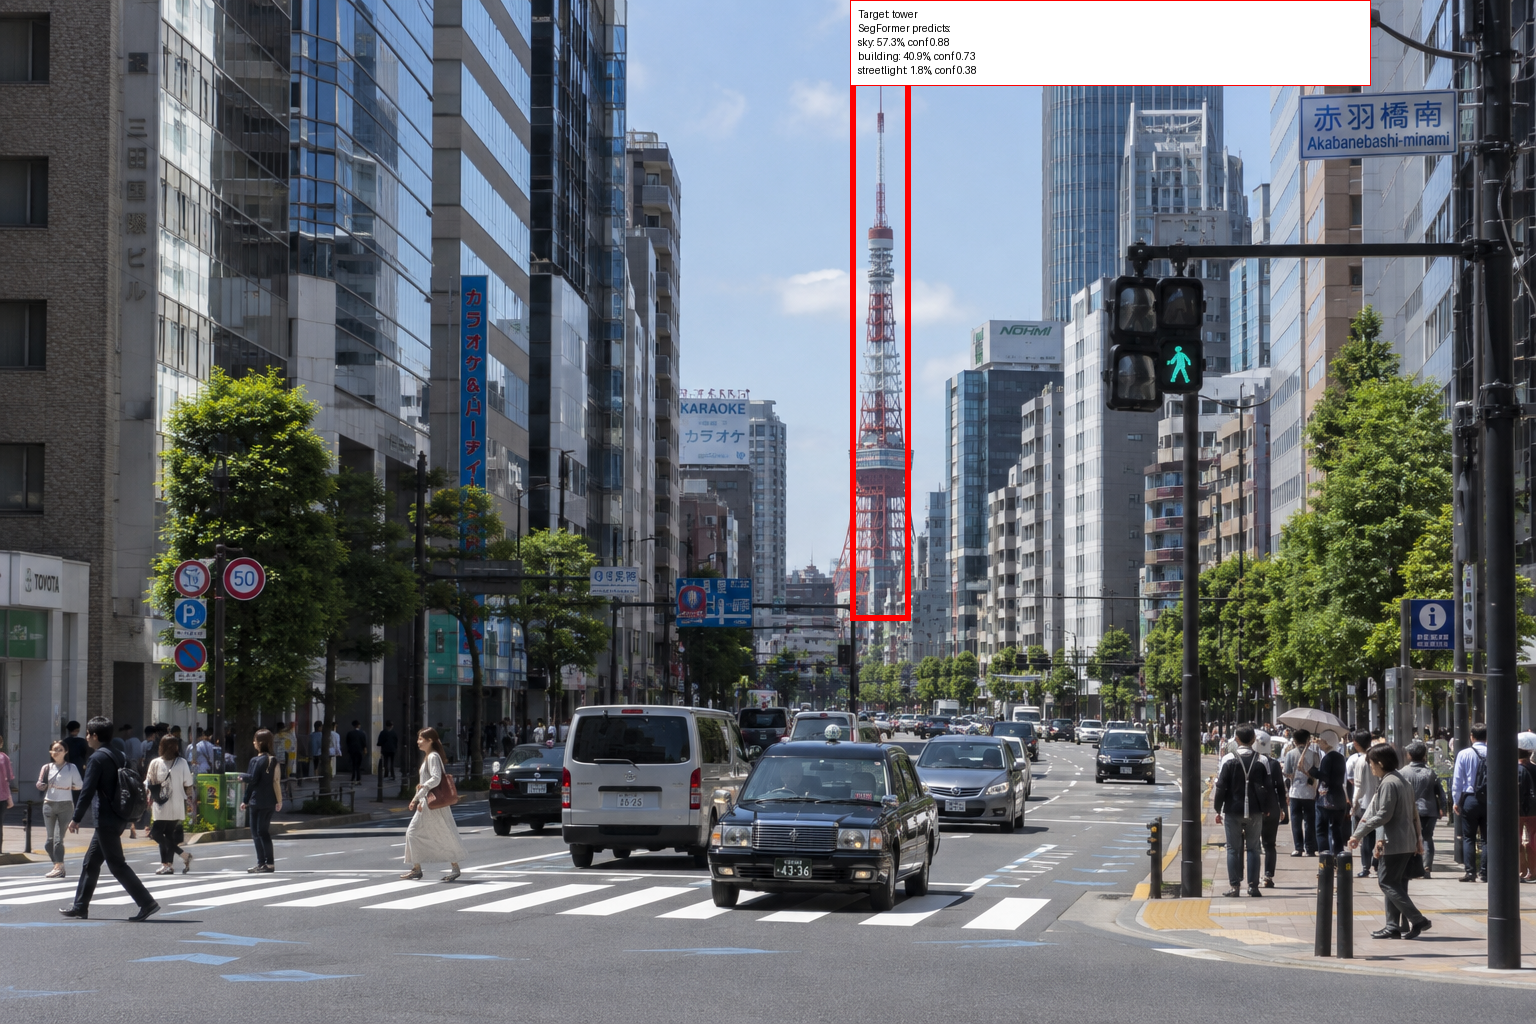
\includegraphics[width=0.85\linewidth]{figures/tower_roi.png}
\caption{ROI analysis for the tower region. The class \texttt{tower} exists in the label set, but the selected region is predicted mainly as \texttt{sky} and \texttt{building}.}
\label{fig:tower_roi}
\end{figure}

This result shows a scale-related failure.
Even though the correct class exists, the model absorbs the thin object into surrounding large classes such as sky and building.
The failure is especially important because the model still gives a high mean confidence.
Thus, confidence alone is not sufficient to detect this error.

\FloatBarrier

\section{Improvement 2: Missing-Target Failure Warning}

\subsection{Attempted Improvement: Crop-Based High-Resolution Inference}

As an attempted improvement, I cropped the tower ROI, enlarged it by a factor of four, and ran SegFormer-B0 again.
The purpose was to test whether the tower class could be recovered by increasing the apparent resolution of the thin object.

However, the result did not recover the tower class.
After crop-based inference, the model predicted 54.7\% of the crop as \texttt{building} and 45.3\% as \texttt{sky}.
The target class \texttt{tower} was still not predicted.
Moreover, the mean confidence increased from 0.8069 to 0.9204.

\begin{table}[H]
\centering
\caption{Crop-based inference result for the tower region.}
\label{tab:tower_crop}
\begin{tabular}{lrr}
\toprule
Predicted class & Ratio & Mean confidence \\
\midrule
building & 0.5469 & 0.8744 \\
sky & 0.4530 & 0.9761 \\
tree & 0.0001 & 0.4467 \\
tower & 0.0000 & -- \\
\bottomrule
\end{tabular}
\end{table}

\begin{figure}[H]
\centering

\begin{subfigure}{0.82\linewidth}
    \centering
    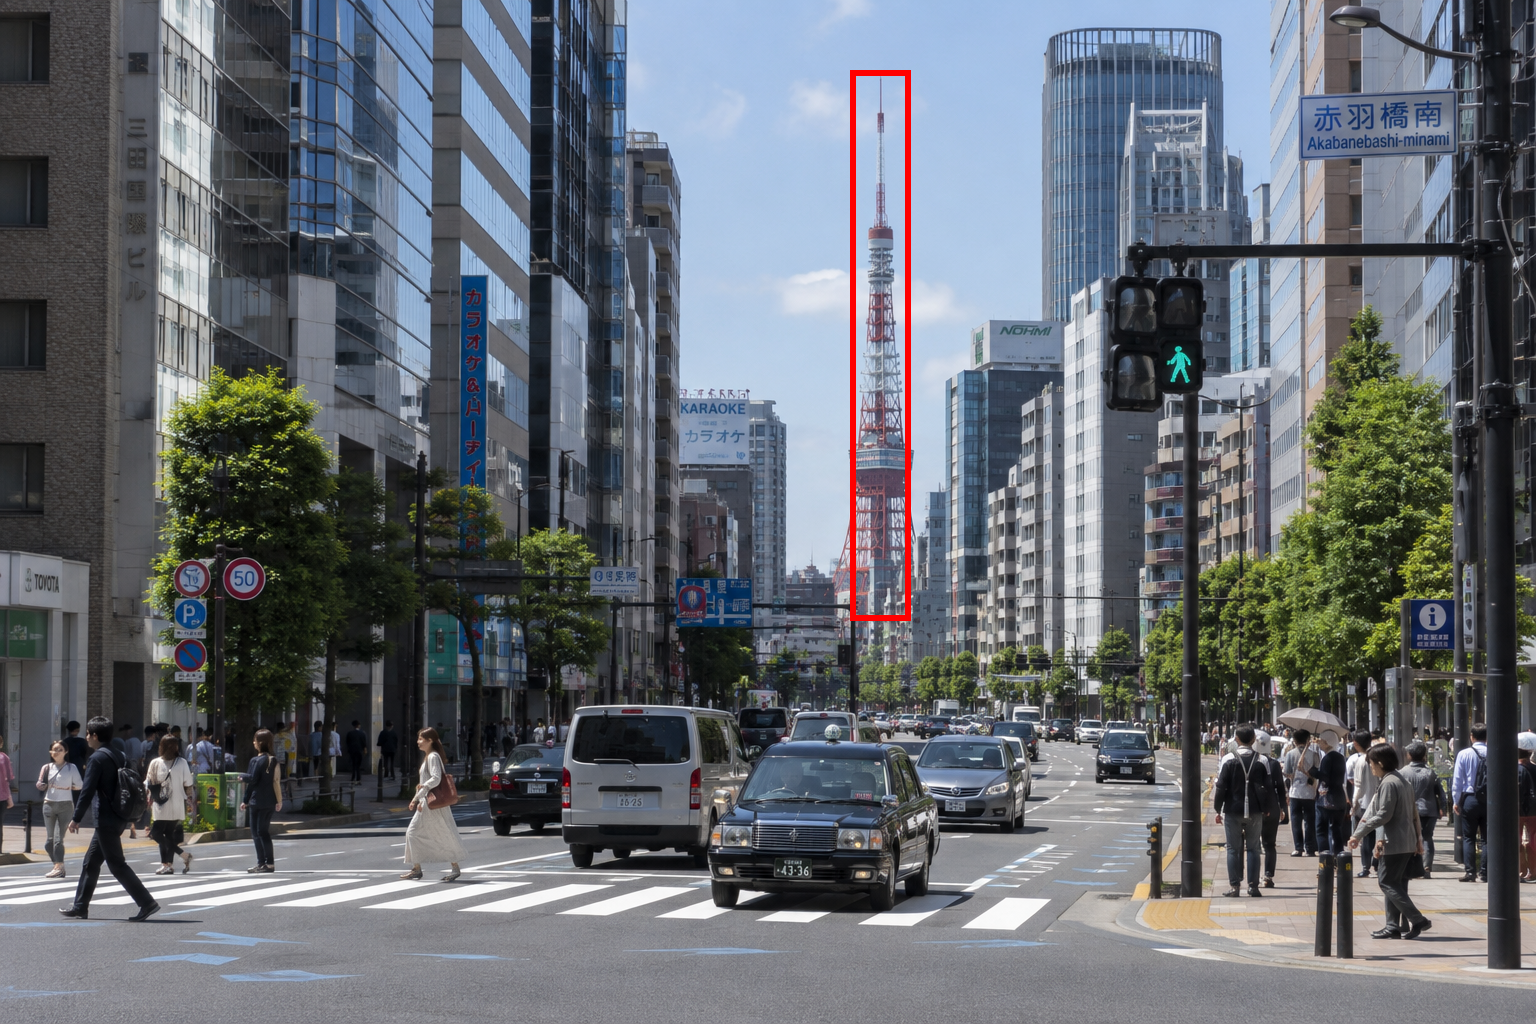
\includegraphics[width=\linewidth,height=0.28\textheight,keepaspectratio]{figures/tower_bbox.png}
    \caption{Original image with the selected tower ROI.}
\end{subfigure}

\vspace{1mm}

\begin{subfigure}{0.42\linewidth}
    \centering
    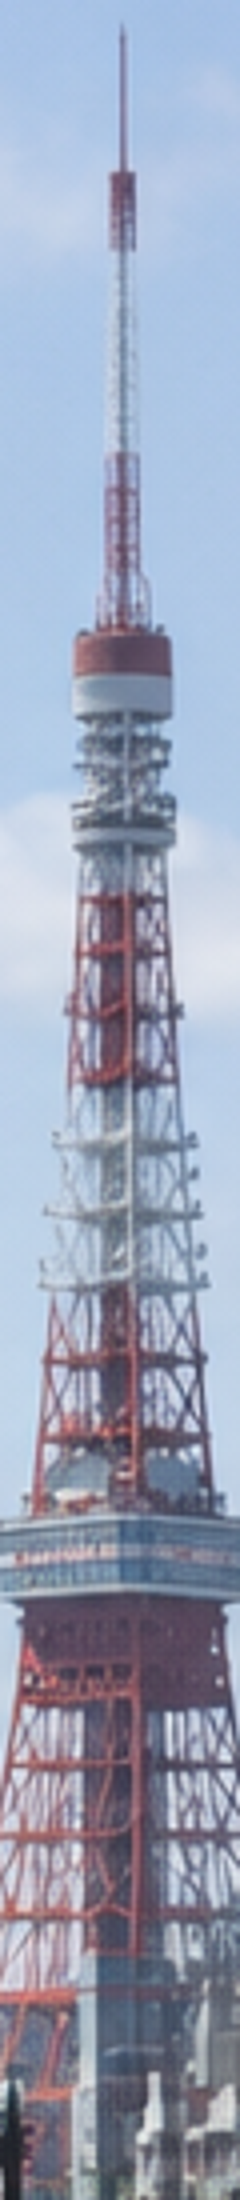
\includegraphics[width=\linewidth,height=0.30\textheight,keepaspectratio]{figures/tower_crop_enlarged.png}
    \caption{Enlarged tower crop used for crop-based inference.}
\end{subfigure}

\caption{Crop-based high-resolution inference experiment. Enlarging the ROI did not recover the \texttt{tower} class.}
\label{fig:tower_crop}
\end{figure}

This negative result is informative.
It shows that the failure is not simply due to low resolution.
Even when the tower is enlarged, SegFormer-B0 still maps it to surrounding scene classes.
This suggests that the model has difficulty representing thin tower-like structures in this context.

\subsection{Proposed Improvement: Missing-Target Warning}

Since crop-based inference did not recover the target class, I added a missing-target failure warning.
The system checks whether the target class exists in the model's label set and whether that class appears inside the selected ROI.
If the target class exists but its predicted ratio is below a threshold, the system warns the user that the object may have disappeared into surrounding classes.

For the tower example, the target class \texttt{tower} exists in the label set, but its predicted ratio inside the ROI was 0\%.
Therefore, the improved system outputs a warning:

\begin{quote}
Warning: the target class \texttt{tower} exists in the label set, but it was not detected in the selected region.
The region was mainly predicted as \texttt{sky} and \texttt{building}.
This may indicate a thin-object or scale-related segmentation failure.
\end{quote}

This improvement does not change the segmentation mask itself.
However, it improves reliability by making a silent failure visible to the user.

\subsection{Baseline vs. Improved System}

\begin{table}[H]
\centering
\caption{Comparison between baseline SegFormer-B0 and the missing-target warning system.}
\label{tab:missing_target_comparison}
\small
\begin{tabularx}{\linewidth}{
    >{\raggedright\arraybackslash}p{0.24\linewidth}
    >{\raggedright\arraybackslash}X
    >{\raggedright\arraybackslash}X
}
\toprule
Method & Output & User interpretation \\
\midrule
Baseline SegFormer-B0
& Predicts \texttt{sky}/\texttt{building} in the tower ROI
& User may overlook the missing tower. \\

Crop-based inference
& Still predicts \texttt{sky}/\texttt{building} with higher confidence
& Failure remains hidden. \\

Missing-target warning
& Warns that \texttt{tower} was not detected
& User notices the possible segmentation failure. \\
\bottomrule
\end{tabularx}
\end{table}

\FloatBarrier

\section{Discussion}

The two failure cases show different limitations of closed-set semantic segmentation.
The vending machine case is a label-space failure: the correct object class is not included in the model's output labels.
The tower case is a scale-related failure: the correct class exists, but the object is too thin and is absorbed into surrounding large classes.

In both cases, the segmentation output alone can be misleading.
The model always produces a class label for every pixel, even when the result is semantically unreliable.
Therefore, the proposed improvements focus on failure detection and visualization rather than changing the model weights.
This is appropriate for a lightweight implementation because it can be added without retraining SegFormer-B0.

\section{Limitations}

This experiment has several limitations.
First, the ROI bounding boxes were manually selected.
A more complete system would need automatic object proposal or user interaction.
Second, the evaluation is mainly qualitative and ROI-based rather than based on full ground-truth segmentation masks.
Third, the proposed warnings do not correct the segmentation mask itself.
They only inform the user when the output is likely to be unreliable.
Finally, the results depend on the ADE20K label set and may differ for SegFormer models fine-tuned on other datasets.

\section{Conclusion}

This report analyzed SegFormer-B0 through practical failure case experiments.
Under normal urban conditions, the model produced reasonable segmentation for large regions such as road, sky, buildings, and trees.
However, two failure cases were observed.
First, vending machines could not be correctly predicted because the class is absent from the ADE20K label set.
Second, a thin tower structure was not detected even though the class \texttt{tower} exists in the label set.
In both cases, the model produced plausible alternative labels instead of explicitly indicating failure.

To improve reliability, I proposed two lightweight warning mechanisms: a class-set-aware OOD warning and a missing-target failure warning.
These improvements do not require retraining and make silent segmentation failures visible to the user.
This shows that even simple failure detection and visualization can improve the practical usability of semantic segmentation systems.

\section{Use of Generative AI}

Generative AI was used to helpthe environmental setup, design the experimental procedure, create and debug Python scripts, and draft the report structure.

\bibliographystyle{plain}
\begin{thebibliography}{9}

\bibitem{xie2021segformer}
Enze Xie, Wenhai Wang, Zhiding Yu, Anima Anandkumar, Jose M. Alvarez, and Ping Luo.
\newblock SegFormer: Simple and Efficient Design for Semantic Segmentation with Transformers.
\newblock In \textit{Advances in Neural Information Processing Systems}, 2021.

\end{thebibliography}

\end{document}
